\chapter{Models and Associated Probes For Proton Spin Structure}
\label{ch:modeling_proton_spin}

\section{Modeling the Proton Structure}

\begin{figure}[ht]
  \centering
  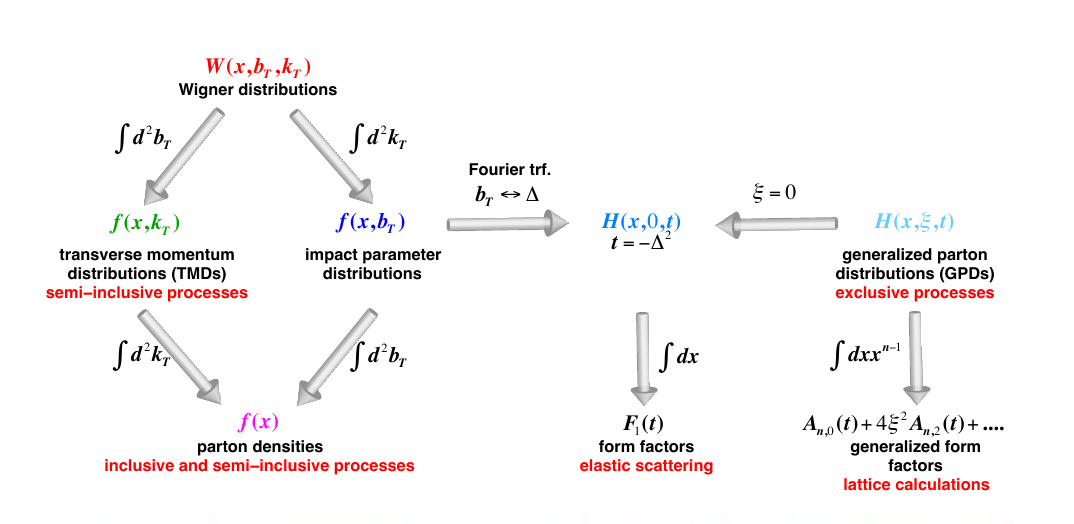
\includegraphics[width=\linewidth]{./figures/pdf_distributions_invariants.png}
  \caption{
    Figure from \cite{Accardi2012}.
  }
  \label{fig:invariants_observables_pdf}
\end{figure}

\section{Structure Functions}
Spin structure overall: \cite{Accardi2012} pp 29-31
Longitudinal spin structure: \cite{Accardi2012} pp 32-43

\begin{figure}[ht]
  \centering
  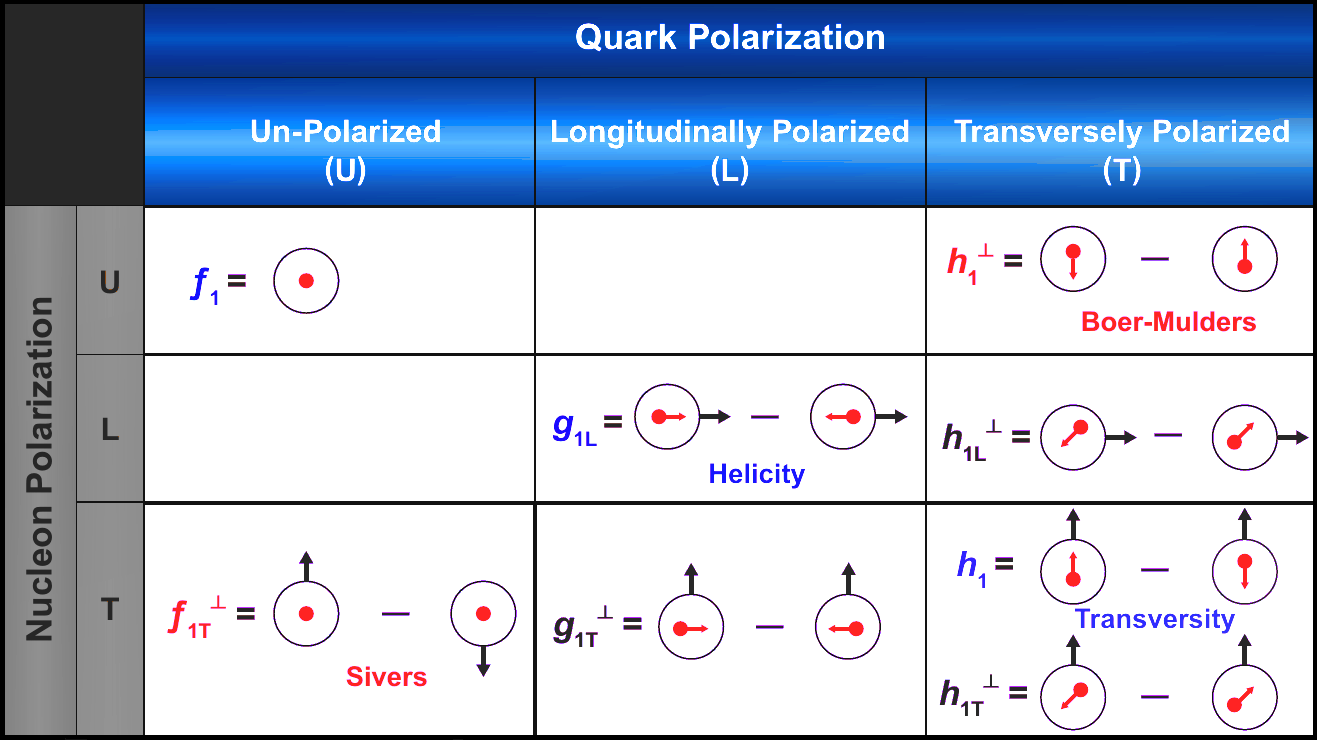
\includegraphics[width=\linewidth]{./figures/leading_twist_polarization_config.png}
  \caption{
    Figure from \cite{Accardi2012}.
  }
  \label{fig:leadings_twist_probes}
\end{figure}

\subsection{Parton Distribution Functions}

\begin{figure}[ht]
  \centering
  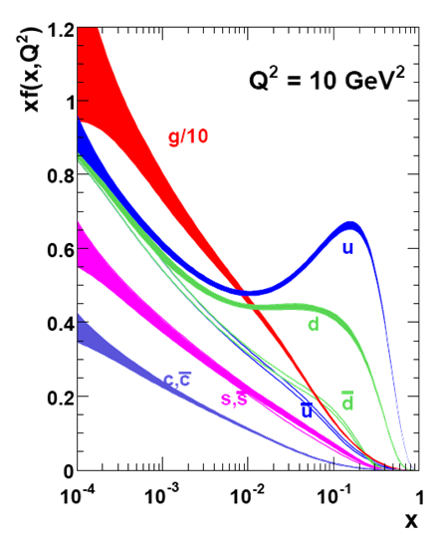
\includegraphics[width=0.5\linewidth]{./figures/quark_kinematics.png}
  \caption{
    Shown: quark kinematics \needcap{} 
  }
  \label{fig:quark_kinematics}
\end{figure}

\subsection{Polarized Parton Distribution Functions}
\label{sec:polarized_pdfs}
Discuss DSSV fits
\subsection{ Proton Spin Decomposition with the Ellis-Jeffe Sum Rule }

Gauge invariant Ellis-Jeffe
\begin{equation}
  \braket{P,{1\over2}|\hat{J_z}|P,{1\over2}}  
 = {1\over2} = {{1\over2}\Delta \Sigma +L_q+J_g}
\label{eq:ellis_jeffe_sum}
\end{equation}

Infinite momentum decomposition:
\begin{equation}
  \braket{P,{1\over2}|\hat{J_z}|P,{1\over2}}  
  = {1\over2} = {{1\over2}\Delta \Sigma +L_q+\Delta g + L_g}
  \label{eq:infmom_ellis_jeffe_sum}
\end{equation}

Quark decomposition:
\begin{equation}
  {\Delta \Sigma} =
  {
    (\Delta u+\Delta \bar{u})
    +(\Delta d + \Delta \bar{d})
    +(\Delta s + \Delta \bar{s})
  }
  \label{eq:quark_spin_decomposition}
\end{equation}

\subsection{ The Spin Asymmetry: An Experimental Probe }
Write in terms of the cross-section of polarized scattering.
\section{ that sweet table from Delia hasch}

\section{Experimental Probes for Proton Spin Structure}
\subsection{Physics Probes for the Proton Spin}

\begin{figure}[ht]
  \centering
  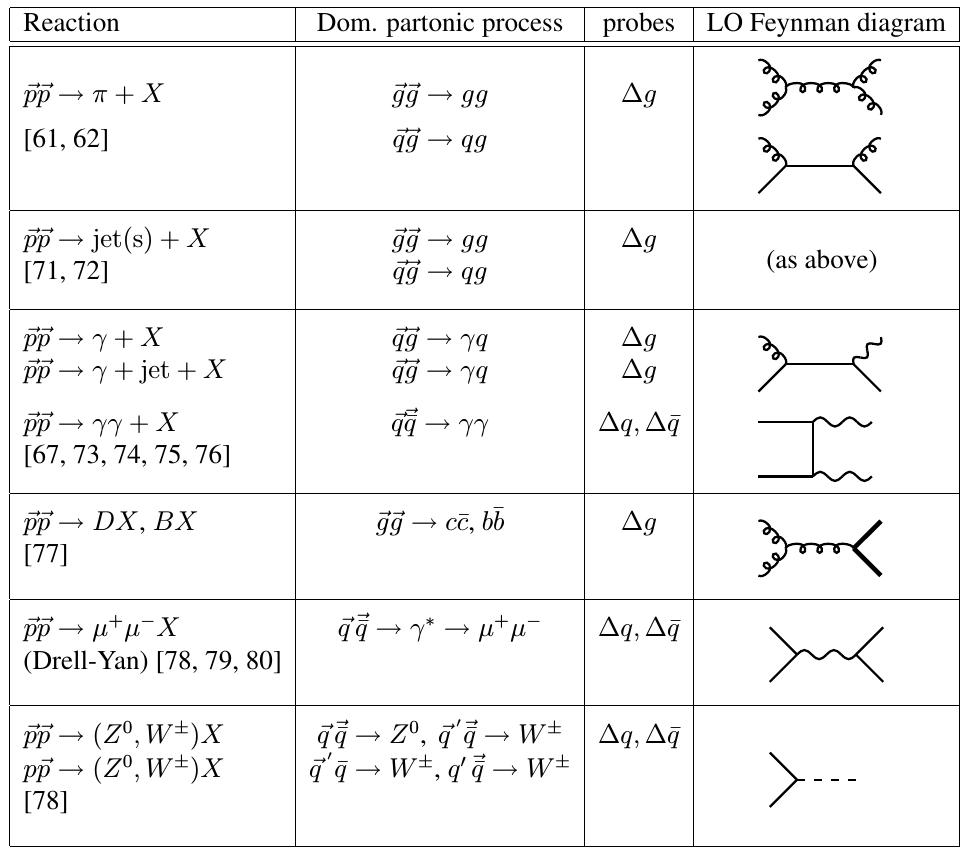
\includegraphics[width=\linewidth]{./figures/spin_probes.jpg}
  \caption{
    A summary of the various probes for longitudinally polarized protons. The
    \textbf{"Reaction"} column summarizes the reaction observed experimentally.
    The \textbf{"Dom. partonic process"} column describes the dominant process
    at the partonic level. The \textbf{"probes"} column shows which proton spin
    structure can be measured with the reaction. Finally, the leading order
    Feynman diagram for the partonic process is drawn. Figure is reproduced
    from: \cite{Aidala2005}.
  }
  \label{fig:spin_probes_masterspin}

\end{figure}

\subsection{W Production}

The standard model tells us that W production occurs through a pure vector-axial
interaction, this implies that the helicity of the parents particles - in
particular $u+\bar{d}\rightarrow W^+$ and $\bar{u}+d\rightarrow W^-$ have fixed
helicities, due to the relativistic final state neutrino (which is not measured,
of course). To visualize the leading order of W production, with regards to the
quark-sea element being probed, the leading order diagrams for the interaction
are shown in Figure~\ref{fig:w_probe_leading_order}~\cite{Aidala2005}

Since $\Delta q$, the polarized parton distribution function can be split into
contributions from valence quarks, and also sea quarks, understanding $\Delta
\bar{q}$ is an important step towards understanding $\Delta q$ better to better
understand the total proton spin.

\begin{figure}[ht]
  \centering
  \begin{subfigure}[b]{\textwidth}
    \centering
    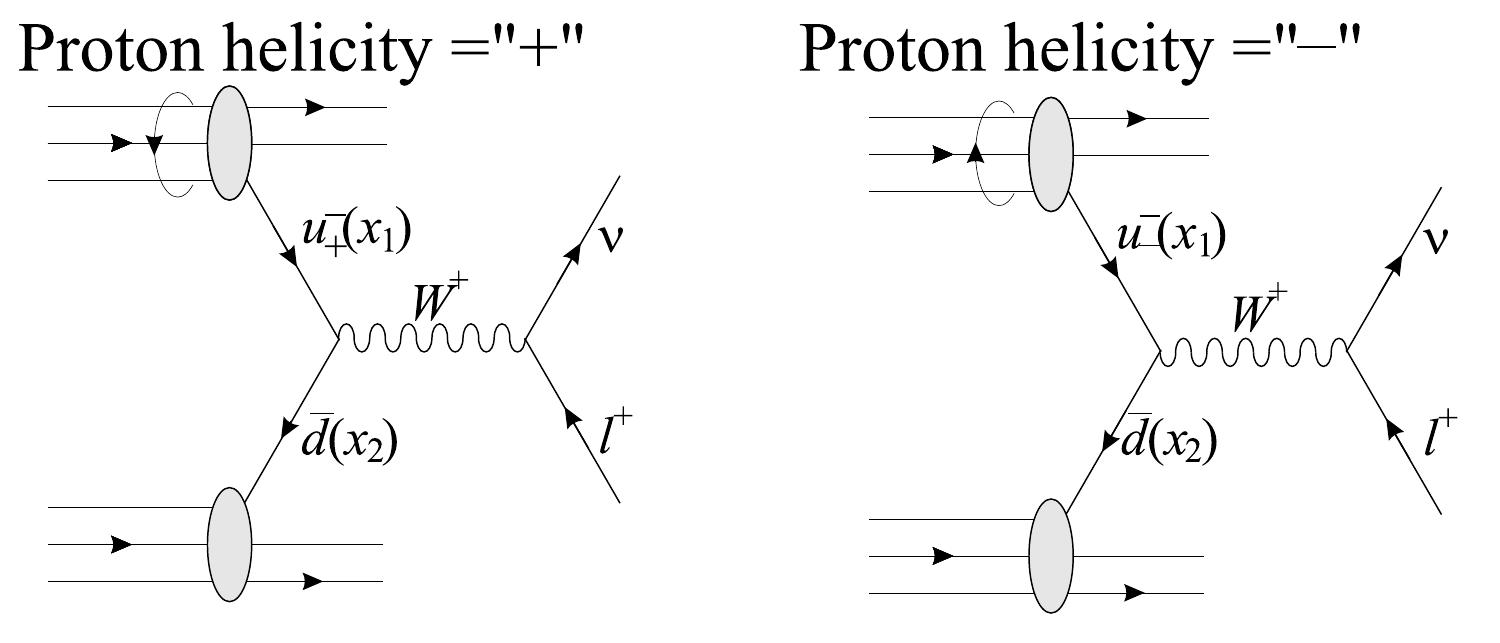
\includegraphics[width=0.8\linewidth]{./figures/w_plus_u_probe.jpg}
    \caption{
      Probe for $\Delta u$ at lowest order.
    }
    \label{fig:u_probe}
  \end{subfigure}
  \begin{subfigure}[t]{\textwidth}
    \centering
    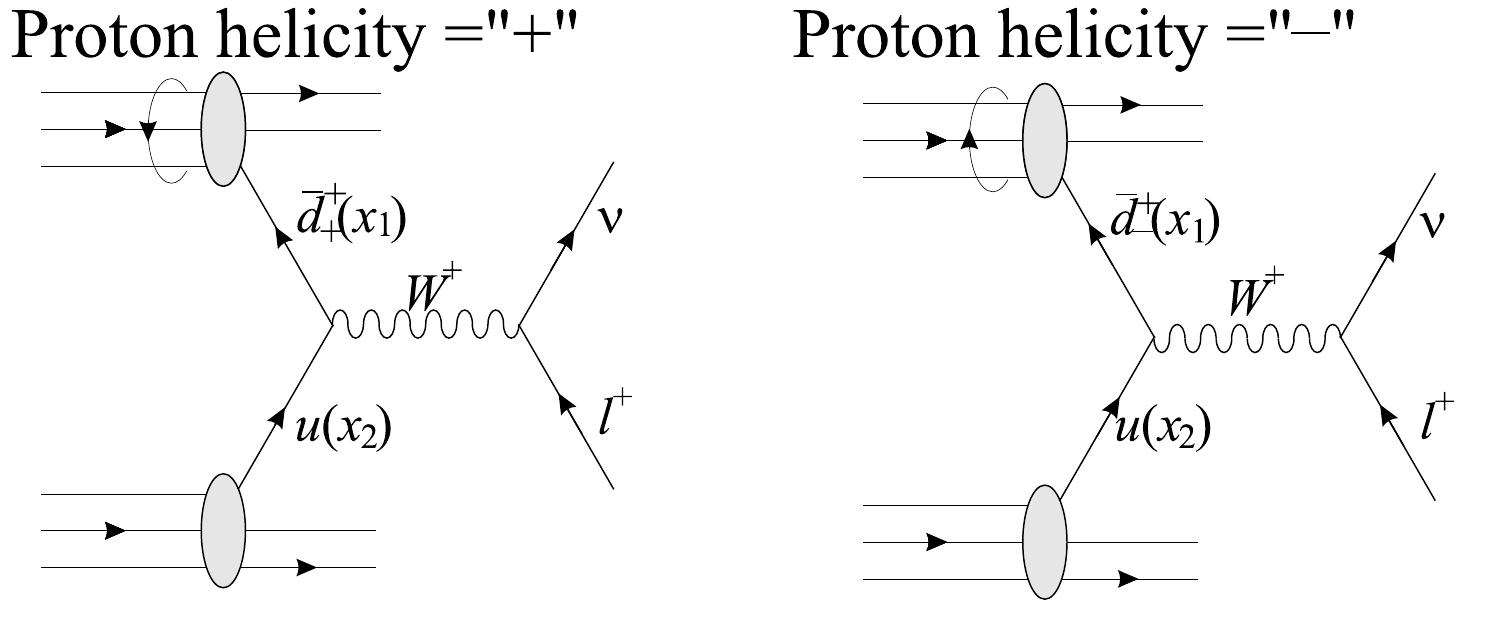
\includegraphics[width=0.8\linewidth]{./figures/w_plus_dbar_probe.jpg}
    \caption{
      Probe for $\Delta\bar{d}$ at lowest order
    }
    \label{fig:dbar_probe}
  \end{subfigure}
  \caption{
    Real $W^+$ production as produced at PHENIX. The helicity of the initial
    state fixes the helicity of the partonic participants due to the
    relativistic final state of the neutrino + the handedness of the W boson.
    $x_1$ and $x_2$ are the momentum fractions of the quarks participating from
    the participant partons~\cite{Aidala2005}. 
  }
  \label{fig:w_probe_leading_order}
\end{figure}

Though both protons in the collision are polarized, the polarization of one
participant proton can be effectively ignored by summing over all polarization
states for one of the two protons. With this assumption, we may construct a
single spin asymmetry for colliding protons by counting difference in the number
of positively and negatively polarized W's produced in collisions, scaled by the
total production:

\begin{equation}
  {{A_L}^W} =
  {{{1}\over{P}}\times{{N_{-}(W)-N_{+}(W)}\over{{N_{-}(W)+N_{+}(W)}}} }
  \label{eq:w_production_asymmetry}
\end{equation}

This is a relatively easy experimental probe to measure (assuming that we can
accurately count events which produced a W, which naturally, is nearly
impossible, as we will see in Section~\ref{sec:sbr}).

As we saw earlier, in Section~\ref{sec:polarized_pdfs}, we can write an
asymmetry in terms of the scattering cross section for the process responsible
for particle yields. These cross-sections were shown to be written in terms of
polarized parton distribution functions, thus, we cut to the chase to write down
the full expression of the theoretical asymmetries for this process in terms of
those parton distribution functions.

The following equations all contain an implied integration over $x_1$ and $x_2$.

For $W^+$ and $u$:
\begin{equation}
  {A_L^{W^+}} = 
  {
    {u_-^-(x_1)\bar{d}(x_2)-u_+^-(x_1)\bar{d}(x_2)}
    \over
    {u_-^-(x_1)\bar{d}(x_2)-u_+^-(x_1)\bar{d}(x_2)}
  }  
  \label{eq:al_u_full}
\end{equation}

For $W^+$ and $\bar{d}$
\begin{equation}
  {A_L^{W^+}} = 
  {
    {\bar{d}_-^+(x_1)u(x_2)-\bar{d}_+^+(x_1)u(x_2)}
    \over
    {\bar{d}_-^+(x_1)u(x_2)+\bar{d}_+^+(x_1)u(x_2)}
  }  
  \label{eq:al_dbar_full}
\end{equation}

Observationally, we see a superposition of \ref{eq:al_u_full} and
\ref{eq:al_dbar_full}, which is expressed as \ref{eq:al_superposition}:

\begin{equation}
  {A_L^{W^+}} = 
  {
    {
      \Delta u(x_1)\bar{d}(x_2)-\Delta \bar{d}(x_1)u(x_2)
    }
    \over
    {
      u(x_1)\bar d(x_2)+\bar(d)(x_1)u(x_2)
    }
  }
  \label{eq:al_superposition_pos}
\end{equation}

For the case of $W^-$, we observe $\bar{d}$ and $u$:
For $W^-$ and $d$:
\begin{equation}
  {A_L^{W^+}} = 
  {
    {d_-^-(x_1)\bar{u}(x_2)-d_+^-(x_1)\bar{u}(x_2)}
    \over
    {d_-^-(x_1)\bar{u}(x_2)-d_+^-(x_1)\bar{u}(x_2)}
  }  
  \label{eq:al_d_full}
\end{equation}

For $W^-$ and $\bar{u}$
\begin{equation}
  {A_L^{W^+}} = 
  {
    {\bar{u}_-^+(x_1)d(x_2)-\bar{u}_+^+(x_1)d(x_2)}
    \over
    {\bar{u}_-^+(x_1)d(x_2)+\bar{u}_+^+(x_1)d(x_2)}
  }  
  \label{eq:al_ubar_full}
\end{equation}

Observationally, we see a superposition of \ref{eq:al_d_full} and
\ref{eq:al_ubar_full}, which is expressed as \ref{eq:al_superposition_neg}:

\begin{equation}
  {A_L^{W^-}} = 
  {
    {
      \Delta d(x_1)\bar{u}(x_2)-\Delta \bar{u}(x_1)d(x_2)
    }
    \over
    {
      d(x_1)\bar u(x_2)+\bar(u)(x_1)d(x_2)
    }
  }
  \label{eq:al_superposition_neg}
\end{equation}

Kinematics of the collision can simplify the equations even further, when at
very forward or very backward rapidities~\cite{Aidala2005}.

\clearpage
\section{Cross Sections and Luminosity}
\begin{itemize}
		\item vernier analysis note intro, equations
		\item summarize the papers on Lumoninosity
\end{itemize}

\clearpage
